\chapter{Implementación}\label{sec:imple}
    \par A partir del análisis y diseño, se realizó la implementación del sistema, los pasos expuestos en la metodología son Reestructuración, Implementación de la nueva Arquitectura, Implementación de nuevas funcionalidades, y un análisis de los problemas

\section{Reestructuración}\label{imp:refactoring}

    El código existente para el bot contenía varios problemas de diseño que hacían compleja su extensibilidad y se pueden revisar detalladamente en la sección de trabajo previo.

    \par Para solucionar estos problemas primero se extrajeron las funcionalidades clave del bot: Obtener información desde la base de datos, recibir \textit{request}, procesar \textit{request} y enviar mensajes. La extracción de información, la recepción y envío de mensajes en sí no presentaba mayores problemas de diseño. 

    \subsection{Cambio en el procesamiento de las Requests}

    \subsubsection{Cambio de procesamiento condicional a parser}
    
        \par Cómo se vio en la sección de trabajo previo, la API de \gls{Telegram} permite varias formas de comunicación. De ellas se utilizan los \textit{websockets}. A partir de aquí, los bots pueden recibir todos los mensajes enviados por el usuario, sin embargo, \gls{Telegram} permite agrupar los mensajes en más o menos 4 modalidades: primero texto, archivos o media adjunta, comandos y los \textit{keyboards}.

        \par En el diseño anterior, como se explicó, se seleccionaron principalmente una manera de comunicación  a través de \textit{inline keyboards}. (sección anterior: En este tipo de comunicación se presentan al usuario una serie de botones que él puede apretar y a partir de los se envía un mensaje al servidor, cuando este es procesado se envía la respuesta al usuario de manera asíncrona). Para poder desarrollar las nuevas \textit{features}, se añadieron comandos, en miras también de procesar texto. Se amplió el diseño para pasar de una decisión condicional a un  \textit{parsing} con \textit{double dispatch}.

        \begin{listing}
            \begin{minted}{python}
                def message_processing(self, t_chat, message, 
                    label=None, question=None ):
                    messages = []
                    if label is None:
                        if message == '/start':
                        messages = [ {"text": 'Hola ...',
                        "keyboard": {}},...]
                        elif message == '/preguntasFrecuentes': ...
                        elif message == '/asistente': ... 
                    Else: ...
                        elif label == 'Process': ...
                        elif label == 'Category': ...
                        elif label == 'Question': ...
                        elif label == 'Helper':  ...
                    
                    for msg in messages:
                        self.send_message(msg['text'],
                        t_chat["id"], msg['keyboard'])
            \end{minted}
             \caption[sistema de procesamiento anterior]{Sistema de procesamiento basado en ifs sobre el tipo de comunicación y la expresión de texto}
        \end{listing}

        \begin{listing}
            \begin{minted}{python}
                def post(self, request: AsgiRequest, *args, **kwargs):
                    update = request.body
                    parser.decode_update(update)
                    return JsonResponse({"ok": "POST request processed"})
                
                    # Parser
                    def decode_update(self, update: bytes):
                            # Se detecta que el update es un mensaje
                            if update.match(message-regex) :
                            return self.parse_expression(message)
                            # Se detecta que el update es una call_bacK_query
                            elif update.match(call_bacK_query-regex):
                            self.parse_expression(label, chat_id)
                            # No see detecta que es el update
                            else:
                                return Updates.UpdateProccesingResult()
            \end{minted}
            \caption[Nuevo Sistema de Procesamiento]{Sistema de procesamiento basado en expresiones regulares y \textit{double dispatch}}
        \end{listing}


    \par Cómo se puede apreciar en este nuevo sistema, el \textit{parser} se hace cargo de determinar que tipo de \textit{update} o actualización que fue recibida desde \gls{Telegram} y a partir de esa detección se pasa la expresión a un \textit{Handler}, este determina que acción debe realizarse y luego llama a la instancia determinada de la acción para que se procese la \textit{request}. Este nuevo modelo es útil principalmente por 5 razones.
    
    \par Mantiene la integridad del procesamiento sin importar si el tipo mensaje de \gls{Telegram} es conocido o no.
    Separa el  \textit{parsing}, de la estructura de la API de \gls{Telegram} del procesamiento de la acción requerida por el usuario en el sistema. Dualidad Parser-Handler.

    \par Permite escalar de forma ordenada el código para recibir muchas nuevas funcionalidades siguiendo un diseño estándar de procesamiento. Esto porque separa la identificación de la acción de su código en particular, estandariza el llamado de las acciones y permite reutilizar patrones de código sin duplicar código. 
    Utiliza un  \textit{parsing}, basado en \textit{regex} y no en comparaciones de \textit{strings}, lo que permite una mayor flexibilidad y robustez del procesamiento.
    \par Da la posibilidad de añadir nuevos tipos de procesamiento de acciones sin cambiar la lógica  de traducción de la API del bot. En otras palabras, para añadir procesamiento de lenguaje natural, no hay que hacer grandes modificaciones al \textit{parser}, solo hay que añadir el \textit{Handler} correspondiente.

    \subsubsection{Creación del \textit{Handler}}
        \par En el sistema anterior todos los comandos tenían su propio bloque de código, principalmente porque solo enviaban mensajes de texto de vuelta al sistema. En el nuevo sistema se deja la tarea de determinar que acción tomar a un \textit{Handler}. Hay dos grandes diferencias entre el \textit{parser} y \textit{Handler} (porque ambos funcionan como un parser).
        
        \par La primera es que el \textit{Handler} se hace cargo de la lógica específica de cada acción de manera estándar, es decir una vez que identifica la expresión de texto, llama a un objeto que contiene la acción a realizar. Uno de los mayores beneficios es que se puede ver claramente cuál es árbol de decisión o el camino de la acción sin entrar en la acción particular, a la vez que permite que las acciones se puedan modificar o extender sin cambiar el llamado predeterminado de los objetos. También hace sencillo extender la funcionalidad. 
        
        \par La segunda, es que cada tipo de mensaje en la API tiene su propia forma de procesarse dada la naturaleza de la comunicación en la API de \gls{Telegram} (objetos de JSON). Por dicha razón cada modo de comunicación tiene su propio \textit{Handler}, esto separa lógicamente la comunicación mediante comandos del texto plano o las callback queries\footnote{Las formas de comunicación responden a diferentes maneras en que un usuario puede enviar mensajes en \gls{Telegram} diferencia estas maneras entregando objetos JSON con propiedades distintas. Si bien hay varias, en la memoria se usan 3: texto plano, \textit{callback queries} y comandos, que se procesan de forma similar al texto plano.}. Esto implica que para extender las maneras de comunicarse basta con agregar un \textit{Handler} que represente esa manera de comunicación. Actualmente se procesan comandos y \textit{callback queries} por lo tanto solo existen esos \textit{Handlers}.

        \par La estructura de un \textit{Handler} es simple, es un objeto que contiene instancias de las diferentes acciones a realizar y define a si mismo, una función handle, que hace el match entre una expresión y la expresión regular que identifica a la misma. Si el match se cumple se llama a la función \mintinline{python}{do_action} de la Acción en Cuestión.

        \par A continuación se muestra como ejemplo el \textit{Command Handler}
        
        \begin{listing}
        \begin{minted}{python}
            class CommandHandler(Handler):
                start_command = StartCommand()
                help_command = HelpCommand()
                unknown_command = UnknownCommand()
                ...

                def handle(self, expression: str, for_id: int) -> None:

                    # expression <-> /start
                    if self.start_command.re.match(expression):
                        self.start_command.do_action(chat_id=for_id)

                    # expression <-> /help
                    elif self.help_command.re.match(expression):
                        self.help_command.do_action(chat_id=for_id)
        \end{minted}
        \caption[Command \textit{Handler}]{Administrador de Comandos a partir del match con expresiones regulares}
        \end{listing}

    \subsubsection{Creación de un modelo OO para respuestas}
        \par Un tercer aspecto es que se extrapoló el concepto de acción a una clase abstracta \textit{Action}, utilizando el módulo abc de Python. El único compromiso de esta clase es realizar una acción. Y a esta clase la extiende dos clases una es \mintinline{python}{Command} y la otra es \mintinline{python}{CallBackQuery}. Que agrupan las funcionalidades típicas de cada forma de comunicación, esto permite al \mintinline{python}{Handler} instanciar varios \mintinline{python}{Commands} o \mintinline{python}{CallBackQueries} por ejemplo y llamar  \mintinline{python}{do_action} en cada una para representar la acción buscada por el usuario.
        Esto también permite diseñar la respuesta a cada acción de manera individual ocultando la complejidad del modelo de interacción.


        \par La última modificación fue, que se creó una clase llamada \mintinline{python}{Objects} con el objeto de imitar el comportamiento de los objetos de la API basados en JSON a objetos de Python. El gran problema lo presentan los objetos compuestos sobre todo en la distinción de tipos, Python ha ido agregando varias herramientas de tipado, pero el estándar de JSON carece de ellas y complica modelos de herencia muy extendidos. Por ejemplo un mensaje contiene dentro un keyboard y el keyboard a su vez contiene una \textit{callback query} a realizarse y ser procesada de vuelta por el sistema. Las detecciones a través de match y regex son muy útles a la hora de procesar el mensaje, pero no tienen el mismo valor a la hora de construirlos, es por eso, que se diseñó un modelo de objetos que pudiera interactuar de manera más sencilla con los objetos de la API de Telegram. Sin embargo, todavía no se logra un modelo completamente funcional que además sea lo suficientemente robusto, como para usarse. Para la creación de estos objetos, se usaron \textit{Typed Dictionaries (TypedDict)} una nueva librería de Python 3.10.

        \par Estos objetos buscan 3 simplificar 3 procesos: la detección de objetos compuestos y sus funcionalidades correspondientes a cada objeto. La transformación de JSON a Python de objetos compuestos. Y por último de Python a JSON.
        \par Se propone investigar si usar el modelo de \textit{serializers} de API rest u otros similares. El principal problema no es la traducción de uno a otro lenguaje, sino la traducción y detección de objetos compuestos.

        \par Como resumen, se pasó de un modelo que contenía toda la lógica de procesamiento de mensajes en la \textit{view} a uno que separa en capas lógicas cada parte de la interacción, aprovecha modelos de herencia y estandariza el comportamiento esperado en cada fase del procesamiento de información.


    \par Se migró de un modelo no extensible (según la lógica de diseño modular) a uno extensible. Se ordenaron en capas la resolución de mensajes y se modularizó y estandarizó la manera de tomar la acción debida en cada situación.

\section{Nuevas Funcionalidades}
    \subsection{Adopción de un framework para taras asíncronas}
    \par Algunas de las funcionalidades comprometidas requerían la ejecución de tareas de forma asíncrona. Particularmente las funcionalidades de subscripción, tales como los recordatorios. Ya que se debía levantar una notificación en el momento indicado para cada usuario. Con este fin, se agregó la librería \gls{Celery} para el manejo de tareas en Python.
    \par \gls{Celery}, es un gestor de tareas o cola de tareas y trabaja en base a un \textit{broker}, eso significa que puede recibir tareas desde diferentes instancias o servicios, y procesarlas de forma eficiente.
    \par La gran ventaja es que para realizar esto se configura una aplicación de \gls{Celery}, esta “entidad” se encarga de enlazar las configuraciones hechas en el código por el desarrollador a un \textit{worker}. Un \textit{worker} es una instancia de \gls{Celery} que funciona como un \textit{thread} o proceso. Entonces \gls{Celery} envía a través del \textit{broker} las tareas que esten configuradas en una APP a un proceso que las ejecuta. En \gls{Celery} se pueden ejecutar tareas directamente, de forma asíncrona o programadas.
    \par A continuación se explica como se usan tareas para lograr hacer funcionar los recordatorios.

    \begin{itemize}
        \item \textbf{Subscripciones:} Una suscripción cómo se explicó en el proceso de diseño es la capacidad que le da el sistema al usuario de elegir de entre una colección de opciones, una o más a alternativas las que suscribirse par obtener información relevante en una cierta frecuencia. Para poder entregar estos mensajes en el momento especificado se crean notificaciones y se requiere un proceso de actualización.
        \item \textbf{Notificaciones:} Una Notificación, en este sistema es un mensaje que debe ser enviado a un usuario en algún momento
    \end{itemize}

    \subsection{Sistema de Suscripciones}
    \par Las suscripciones son un sistema de 3 pasos: primero se crea una suscripción, más una notificación asociada y luego el sistema revisa periódicamente las notificaciones almacenadas para decidir cuáles corresponden a ser enviadas. Finalmente modifica la notificación para que almacene el próximo envío.
    Para revisar periódicamente las notificaciones, se establecieron tareas recurrentes con \gls{Celery} que revisan la base de datos manera constante y en el caso de encontrar una colección de notificaciones que deben enviarse hoy, se envían. 
    De este modelo el envío de las notificaciones se realiza por parte del gestor de tareas.
    Esto da un comportamiento dual en el que las suscripciones se realizan de manera síncrona (por el usuario) y las notificaciones se envía de forma programada (por el sistema).
    \par La configuración de \gls{Celery} es simple, ya que se realiza una breve configuración inicial y las tareas simplemente se identifican con @decorators\footnote{ Los @decorators de Python, son azúcar sintáctico, en el que nombre del \textit{wrapper} se corresponde con una función del mismo nombre, esta última recibe cómo parámetro la función que el @decorator acompaña.} de Python  
    El código queda más o menos así:
    \begin{listing}
    \begin{minted}{python}
        app = Celery('API')
        app.config_from_object('django.conf:settings', namespace='CELERY')
        app.autodiscover_tasks()

        app.conf.beat_schedule = {
            # Executes every Monday morning at 7:30 a.m.
            'add-every-minute': {
                'task': 'tasks.send_today_notifications',
                'schedule': crontab(minute=1)
            },}

        @shared_task
        def send_today_notifications():
            notifications = Notification.get_today_notifications()
            messages = [] #[{"text": '', "keyboard": {}}]
            
            for notification in notifications:
                msg = markup_clearner(f'{notification.msg}')
                try:
                    notf_susc = notification.subscription
                    notf_chat = notf_susc.chat
                    print(notf_chat)
                except:
                    notf_chat = None
                notf_message = {'text': msg, 'keyboard': {}, 'chat': notf_chat}
                messages.append(notf_message)

            for msg in messages:
                if msg['chat'] is None:
                    continue
                async_send(msg['text'], msg['chat'], msg['keyboard'])
    \end{minted}
    \caption[Sistema de notificaciones]{Sistema de notificaciones basado en \gls{Celery}}
    \end{listing}

    \par Algunas notas sobre el sistema de Subscripciones. Para lograr programar tareas se utiliza un módulo de \gls{Celery} que se ejecuta como un proceso paralelo llamado Celery beat. Además los resultados de las tareas y las tareas programadas se guardan en la base de datos. De esta forma hay al menos 2 procesos paralelos en ejecución un \textit{worker} de la aplicación y beat el programador que hace uso de la db.

\newpage
\section{Cambios en Diseño}

    \subsection{Cambios en la arquitectura}

    \begin{figure}[h!]
        \centering
        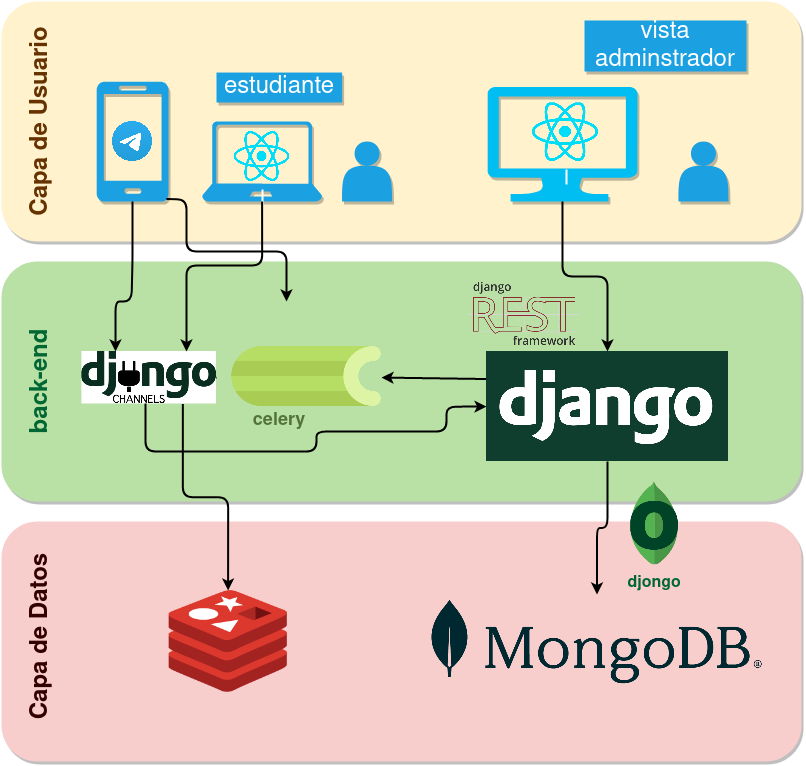
\includegraphics[width=\textwidth]{media/diagramas/arquitectura/nueva_arquitectura.png}
        \caption[Nueva arquitectura]{Diagrama de arquitectura del nuevo sistema}
        \label{fig:arc-new}
    \end{figure}


    \par La nueva arquitectura cómo se puede apreciar en el diagrama integra:
    \begin{itemize}
        \item \textbf{La Base de Datos (MongoDB):}  En la base de datos se almacenan los datos de autenticación, la información de la aplicación, el contenido de subscripción, las preferencias de los usuarios y las tareas.
        \item  \textbf{Backend Django:} Contiene la lógica del servicio de contenido, también configura y programa las tareas (de manera manual una vez). Se comunica a través del broker con la cola de tareas.
        \item \textbf{Broker de Mensajes (Redis):} Sincroniza a través de mensajes diferentes módulos de la aplicación
        \item  \textbf{API Telegram:} Servicio externo proporcionado por \gls{Telegram} que permite la comunicación entre la app y los usuarios del bot (que son por defecto usuarios de telegram).
        \item  \textbf{El Front web:} Sirve tanto como plataforma de información como centro de control de para los staf de la mesa de ayuda.
        \item \textbf{Celery:} Maneja las tareas programadas, asíncronas y directas desde la aplicación.
    \end{itemize}
    
    \subsection{Cambios en los módulos}

    \begin{figure}[h!]
        \centering
        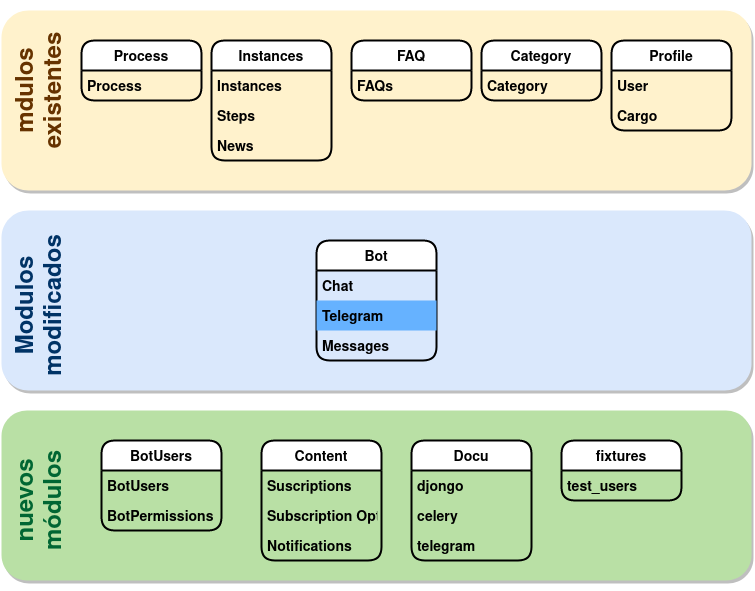
\includegraphics[width=\textwidth]{media/diagramas/arquitectura/arc-logica.png}
        \caption[Nueva arquitectura]{Diagrama de arquitectura del nuevo sistema}
        
    \end{figure}
  

    Módulos ya existentes
    \begin{itemize}
        \item Process, correspondiente al módulo de procesos descritos anteriormente.
        \item Instances, correspondiente a las instancias de cada proceso.
        \item FAQ, el cual aborda las preguntas frecuentes asociadas a un proceso.
        \item Category, asociado a las categorías de una pregunta. Esta aplicación es utilizada por el bot y se describe con más detalle en la sección 5.3.
        \item Profile, correspondiente al manejo de usuarios(as) de la aplicación Web.  
    \end{itemize}

    Módulo modificado
    \begin{itemize}
        \item Bot, correspondiente a la implementación del bot de \gls{Telegram} de esta solución. Se añaden los submodulos de: \gls{Telegram} y task. En tasks, se almacena las nuevas tareas periodicas del sistema, aunque pueden agregarse en cualquier parte del backend. En el modulo de \gls{Telegram} se integra la nueva lógica de \textit{parser}, \textit{Handler}, acciones y objetos.
    \end{itemize}
    
    Modulos nuevos
    \begin{itemize}
        \item BotUsers, corresponde al manejo de los usuarios(as) del Bot.
        \item Content, correspondiente al manejo de las suscripciones y otras funcionalidades de contenido.
        \item Docu, que añade la documentación del sistema y los procesos realizados
        \item Fixtures, que añade datos de prueba para poblar el sistema.
    \end{itemize}

\section{Problemas de compatibilidad}
    \par Dentro del desarrollo del sistema, dadas las tecnologías heredadas, y decisiones de diseño anteriores, al implementar nuevas tecnologías hubo varios problemas de compatibilidad, los más relevantes se detallan a continuación.

    \par \gls{Django} que es el \textit{framework} de desarrollo web en el que está desarrollado el proyecto, funciona con un sistema llamado Object Relationship Mapping (\gls{ORM}), que lo que hace es traducir operaciones de objetos de \gls{Django} a queries en la base de datos relacional. Esto en general era parte de desarrollo de las aplicaciones en frameworks como spring de java, aun es necesario realizar este tipo de adecuaciones, para trabajar con los resultados salientes de la base de datos. Esta funcionalidad clave de \gls{Django} da una enorme simplicidad y versatilidad al código. Por otro lado Mongo es una base de datos no relacional, si bien se puede integrar a Python con varias librerías integrarla con el \gls{ORM} de \gls{Django} no es tan sencillo. De hecho, en general hay conectores a base de datos pero no algo similar al \gls{ORM}. En ese sentido \gls{Djongo} es un proyecto que logra soslayar esta dificultad, con lo que ellos llaman un \gls{ODM} un \textit{Object Document Mapping}. Ahora como todas las operaciones en Mongo son operaciones de documentos y no de tablas, la traducción no siempre es perfecta, y eso implica que funcionalidades como una migración para cambiar el tipo de una tabla por ejemplo no solo no sean necesarias sino imposibles. Ya que mongo no necesita ni tiene un método para cambiar el tipo de tabla, en realidad, nada asegura que un documento dentro de la misa colección tenga el mismo formato que otro, por esto se puede modificar los modelos de \gls{Django} en vivo y el cambio se ve reflejado de manera directa sin migraciones.
    
    \par Por otro lado para lograr la mayor compatibilidad posible \gls{Djongo} crea un súper set al módulo models de \gls{Django} para incluir algunas estructuras interesante como modelos embebidos, arreglos entre otros.

    \par Uno de los grandes problemas es que \gls{Django} por \textit{default} crea un identificador de tipo \textit{int}, que se puede reemplazar manualmente por cualquier otro, pero en el caso de \gls{Djongo} se agrega usualmente por temas de compatibilidad, sin embargo, esto no ocurre el total de las veces, de hecho, para todos los modelos nuevos que se crearon en el proyecto para algunos funcionaba y para otros no aleatoriamente, esto causo un error muy complejo de resolver porque fue muy difícil de identificar. Al mismo tiempo complicó la administración de módulos o librerías que funcionaban con el \acrshort{ORM} de \gls{Django} como la vista de \textit{Admin} y \gls{Celery}.

    \par Para resolverlo se probaron muchas soluciones, pero finalmente, lo que se hizo fue extender la clase Models por default de djongo-django, para que incluyera automáticamente el identificador id que ahora es de tipo uuid. Esto solucionó, los problemas de compatibilidad con el administrador y otros servicios similares.
    
    \par Para \gls{Celery} y otros servicios, la solución fue no pasar por \gls{Django}, \gls{Celery} se conectó directamente a Mongo como base de datos a través de una librería experimental, pero la forma de guardar los elementos la hace imposible de manejar con el \acrshort{ORM} de \gls{Django} o con las vistas de administrador. Por lo tanto para poder administrar y revisar las tareas se requirió instalar \gls{Flower}. Esta librería permite hacer el seguimiento a los eventos que \gls{Celery} expone (lo que se debe configurar) y eso permite hacer un seguimiento de las tareas de la sesión, para las tareas programadas en otro arranque de \gls{Flower} y \gls{Celery}, se hace necesario revisar directamente en la base de datos, ya que tampoco tienen permanencia los mensajes en el \textit{Message Broker} en este caso \gls{Redis}.
    
    \par La suma de todos estos problemas hizo que fuera difícil configurar el proyecto, hacer trazabilidad de los errores, y una vez configurador entender por qué ciertas líneas de código funcionaban para ciertos objetos en la base de datos y para otros no.
    
    \par Sumado a esto \gls{Celery} y \gls{Djongo} son librerías bastantante activas, de hecho \gls{Celery} cambió completamente su documentación de dominio hace solo unos meses, las últimas \textit{releases} son del 2021, aunque ha habido convenciones anuales por Varios años. Por otro lado \gls{Djongo} se actualizó de ser una librería libre, a tener una versión de pago para empresas, a dar soporte, incluso ahora se ofrecen otros servicios \textit{cloud} usando \textit{Mongo Atlas} entre otros.
    
    \par Esto hace que mantener el proyecto requiera de estar en constante revisión de los recursos utilizados, ya que las dependencias están en constante actualización. Esta fue una de las lecciones más importantes del proyecto, a la vez que uno de los mayores desafíos.

\section{Resumen}

    \par Inicialmente se propusieron el análisis y reestructuración de código existente para soportar las nuevas funcionalidades. Además dentro de las nuevas funcionalidades se propuso creer un sistema que permitiera ser personalizado y confiable, a partir del análisis del \acrlong{f}, se añadieron variables sobre la privacidad, parametrización y eficiencia.
    
    \par A partir de diseño y de las evaluaciones se priorizaron las funcionalidades más complejas en términos de implementación, menos controversiales y con más apoyo de los usuarios. Esto derivó en que no se realizaran cambios para agregar información a las respuestas y mejorar el modelo de feedback del usuario. Esto sumado a las \textit{features} que requieren análisis de privacidad usualmente requieren especificar más de una vía de acción.
    
    \par A modo general se cumplió con lo planificando priorizando los cambios de mayor envergadura. Se corrigieron bugs y se mejoró el estilo de procesamiento del bot, para permitir dejar un sistema extensible.